\pdfoptionpdfminorversion=7
\documentclass[sigconf, table]{acmart}

\usepackage{array}
\usepackage{comment}
\usepackage{graphicx}
\usepackage{csquotes}
\usepackage{balance}
\usepackage{setspace}

\usepackage{listings}
\usepackage{subcaption}

\usepackage{standalone}

\lstset{ %
language=C++,                % choose the language of the code
basicstyle=\ttfamily\footnotesize,       % the size of the fonts that are used for the code
columns=fullflexible,
numbers=left,                   % where to put the line-numbers
numberstyle=\footnotesize,      % the size of the fonts that are used for the line-numbers
stepnumber=1,                   % the step between two line-numbers. If it is 1 each line will be numbered
numbersep=5pt,                  % how far the line-numbers are from the code
%backgroundcolor=\color{codeBG3},  % choose the background color. You must add \usepackage{color}
showspaces=false,               % show spaces adding particular underscores
showstringspaces=false,         % underline spaces within strings
showtabs=false,                 % show tabs within strings adding particular underscores
frame=single,           % adds a frame around the code
tabsize=2,          % sets default tabsize to 2 spaces
captionpos=b           % sets the caption-position to bottom
breaklines=true,        % sets automatic line breaking
breakatwhitespace=false,    % sets if automatic breaks should only happen at whitespace
keywordstyle=\color{blue},       % keyword style
  %language=Octave,                 % the language of the code
  otherkeywords={SearchVar,MV,TSS,tileExpr,Search,tFunc...},           % if you want to add more keywords to the set
  numberstyle=\tiny\color{black}, % the style that is used for the line-numbers
  rulecolor=\color{black},
escapeinside={<@}{@>}
}
\definecolor{ForestGreen}{RGB}{34,139,34}
\newcommand{\todo}[1]{{\textcolor{red}{{\tt{TODO:}}\,\,#1 }}}
\newcommand{\nc}[0]{\todo{cite}}
\newcommand{\an}[1]{{\textcolor{blue}{Author's Note: #1}}}
\newcommand{\ttt}[1]{{\texttt{#1}}}

\newcommand{\FormatDecisions}[0]{{\texttt{FormatDecisions}}~}
\graphicspath{{.}{ScoreValidity}}

\usepackage[subtle]{savetrees}

\title{Data Layout Optimization in RAJA}


% \author{Brandon Neth}
% \affiliation{%
% 	\institution{University of Arizona}
% 	\city{Tucson}
% 	\state{AZ}
% 	\country{USA}}
% \email{brandonneth@email.arizona.edu}

% \author{Thomas R.W. Scogland}
% \affiliation{
% 	\institution{Lawrence Livermore National Laboratory}
% 	\city{Livermore}
% 	\state{CA}
% 	\country{USA}}

% \author{Bronis R. de Supinski}
% \affiliation{
% 	\institution{Lawrence Livermore National Laboratory}
% 	\city{Livermore}
% 	\state{CA}
% 	\country{USA}}

% \author{Michelle Mills Strout}
% \affiliation{%
% 	\institution{University of Arizona}
% 	\city{Tucson}
% 	\state{AZ}
% 	\country{USA}}




\begin{document}

\begin{abstract}
%In a world of ever-increasing diversity of computing platform, performance portability is of critical importance. 
%Especially in high performance computing contexts, the portability of optimizations balancing parallelism and data movement are key. 
%Such optimization portability was developed in RAJALC, an extension of RAJA incorporating the loop chain abstraction.
%This work created an inter-loop context for the purpose of schedule optimizations like loop fusion and overlapped tiling.
%While RAJALC enabled the portable specification of complex schedule changes, it left unleveraged a significant factor on performance: data layouts.
%\todo{Brandon, I am not sure we want to bring up RAJALC.  Unless the symbolic execution in RAJALC is how you
%are doing the data layout specifications and layout changes as well?  Or developing the model maybe?  The
%connection needs to be made explicit.  I take a guess in the draft intro.}



The layout of data in memory is a key consideration in high performance computing applications.
From reducing cache and page misses to relieving pressure on memory bandwidth and avoiding inter-process communication, good data layout improves performance at all levels of an application.
RAJA, a C++ performance portability library, incorporates the layout of an application's data into its definition.
Thus, a developer can try out different layouts without major refactoring costs.
However, some applications benefit from changing the data layout mid-computation to facilitate better locality.
Implementing such a mid-computation layout change in RAJA can improve performance, but is laborious to implement and lacks portability.
This work remedies RAJA's shortcoming by introducing a lightweight, declarative API for changing data layouts between computations.
Also, we present an automated layout decider that dynamically estimates performance using the loop bounds and data access order as input. 
These systems work together, meaning the decider \enquote{fills in} layout choices not made by the user.
This allows the user to specify as much or as little of the layout information as they please and still obtain the performance benefits of changing data layouts.  
Further, our system is built directly into the RAJA library, meaning that no additional build steps are required.
We evaluate our system on four benchmarks, where it achieves similar performance improvements to hand-implemented optimizations.
\end{abstract}



\maketitle

\section{Introduction}

How data is stored and accesses has always been recognized to have a significant impact on performance. 
On a typical cache-based system, iterating through a two-dimensional array in column-order when data is 
stored in row-order can lead to a \todo{how much} slowdown 
\todo{cite... what if we just used our own results here? The verification of the traversal order stuff will show this}.
Although mechanisms such as compiler optimizations (loop permutation/interchange) 
and data layout policies like those in Kokkos \cite{edwards2014kokkos} and RAJA \cite{hornung2014RAJA} have the potential to align data layout with computation schedules, they become difficult to automate and laborious to manage by-hand as the number of loops and arrays grow.
\todo{Probably a good idea to refer to existing solutions to this problem as my familiarity with the literature grows}

In this paper, we present an approach for exposing data layout decisions to the programmer in the C++ performance portability library RAJA.
% FIXME: might want to say "C++ portable parallel library RAJA", parallelism is a key goal for RAJA
The presented API allows the programmer to specify as many data layout decisions in a sequence of data-sharing loops (otherwise known as a loop chain~\cite{krieger2013loop}) as they choose.
Then, using a portable cost model based on microbenchmarking, our system identifies any remaining layout changes that will improve performance.  

% HAPPY: I really like this concrete example for motivating the performance benefit.
Figure~\ref{IntroExample} shows how important good data layout is. 
The BadLayout column shows the execution time for a matrix multiplication where the three arrays are laid out opposite of their access order. 
The GoodLayout column shows the execution time for the same matrix multiplication when the arrays are laid out to match their access order.
Finally, the LayoutChange column shows the execution time of code that changes the layout from the bad layout to the good one.
As the graph shows, there is significant performance improvement ($1.49\times$ speedup) simply by changing the data layout, and the cost of performing the layout change is small ($1.42\times$ speedup when including conversion time). 

\begin{figure}
	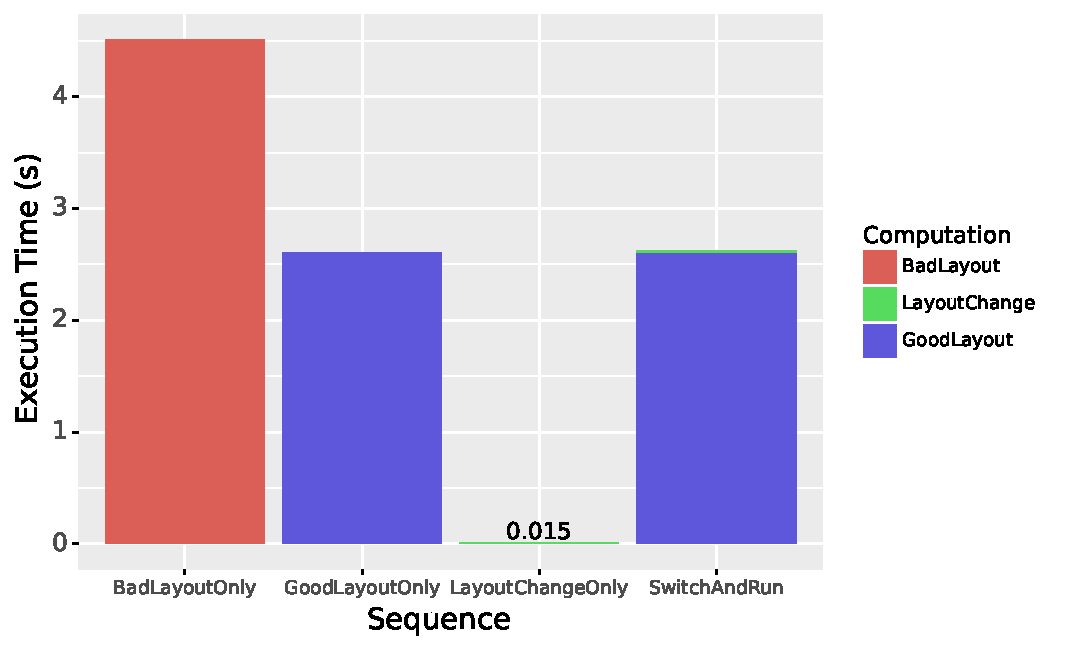
\includegraphics[width=0.7\columnwidth]{ScoreValidity/IntroExampleGraph.pdf}
	\caption{Execution time for matrix multiplication using optimal and non-optimal data layouts and execution time for converting from non-optimal to optimal.}
	\label{IntroExample}
	\Description[Matrix Multiplication Execution Time for Different Layouts]{A bar plot showing a "Bad Layout" column with execution time greater than the "Good Layout" and "Layout Conversion" columns combined.}
\end{figure}


% \todo{Brandon, also we need to figure out how parallelism is related to this work, if at all.  It seems like the
% data layouts are important because of the sequential array access order.  The below introduction does NOT
% bring in parallelism yet due to my lack of understanding on this point.}

% \todo{RUNNING EXAMPLE: A paragraph showing an example sequence of loops 
% (2 would be sufficient) 
% where you can show a scatter plot of performance based on different data layout choices.  
% The Listing 1 example of 3MM would probably work.
% The main points to make
% are that which data layout is selected has a significant performance impact and that sometimes
% it is worth the cost of dynamically changing the data layout between computations.}

Although controlling data layout is quite important, the options programmers have to control
data layouts in coordination with loop schedules have limitations.

Compiler optimizations such as loop permutation have been developed to change loop
schedules so that a loop traversal order better aligns with data layout.
However, general purpose compilers (1) have difficulties analyzing for the relationship between
data layout and schedule due to things like aliasing and lack of multidimensional arrays in 
C/C++ languages, (2) do not generally expose fine-grained data layout or loop optimization
controls to users, and (3) typically do not optimize across multiple loops well.
\todo{Michelle: My understanding is that also you can't optimize two accesses at once with this method, bc changes to optimize one may un-optimize the other. Is this worth mentioning as well?}
\todo{We should have citations for these limitations probably}
% DATA: I thought of "Pointer Analysis: Haven't We Solved This Problem Yet?" from 2001, but there
% are probably more recent papers talking about how difficult precise pointer and alias analysis is
% for C/C++ programs.  I recommend searching for that one.
% For lack of fine-grained controls could you say something like "thus the proposals to potentially
% add loop transformation specs to pragmas in OpenMP and cite the Michael Kruse paper that
% was in the same IWOMP as one of our loop chain transformation papers (Ian's or yours, don't remember).
% It seems like the problem of not optimizing across multiple loops was a key part of the big picture
% problem in many of those papers we looked at in the 620 class.  An email I sent on Aug 3, 2020
% has some notes on potential related work.

Data layout policies provided in libraries like Kokkos or RAJA
and programming languages like Chapel~\cite{diaconescu2007approach} give
programmers control over the data layout of multi-dimensional arrays, but do not 
provide assistance for switching between data layouts between computations \todo{confirm for Kokkos}
nor help with selecting the most effective data layout strategy for a sequence of computations.

\todo{this paragraph seems to echo the above. I'm going to try to make it address the limitations better. Or change the flow.  MMS agrees.  I think in the above paragraph you could summarize what a programmer
would have to do using that control over data layout to get the benefits you show in Figure 1.
Then talk more about the problem being the programmer has to make all of the data layout decisions,
there is potentially a large space of possible solutions, and it is non-trivial to try out all possible options.}
In this paper, we present an extension to the RAJA C++ library that enables a programmer
to specify the data layout for each multi-dimensional array before each 
computation\footnote{Since the control is completely exposed, an autotuner could also try out different options.}.
\todo{Show the api for specifying the best performing data layout strategy
for the RUNNING EXAMPLE.}
However, the programmer does not have to specify all data layout information, because
we also present a run-time performance model based on microbenchmarking that is
then fed into an Integer Linear Programming problem to make all of the data layout decisions
that the programmer has not made.
The performance model and ILP solver can run dynamically or ahead of time.

This paper includes the following contributions:
\begin{itemize}
\item An API in RAJA for specifying data layouts and data layout transformations.
\item A performance model to select a data layout and data layout transformation strategy for 
         a loop chain.
\item An evaluation of the performance model that shows ...\todo{how often is it right on how many architectures}
\item An optimization for reducing the amount of micro-benchmarking needed.
\item SLOC and performance results for the resulting data layouts on 3MM, ...
\end{itemize} 


%%%%%%%%%%%%%%%
\section{RAJA and RAJALC}

\begin{figure}
	\begin{lstlisting}[
		caption={The running example for this paper. 
		We start with an implementation of the 3MM kernel (E = A * B, F = C * D, G = E * F) in RAJA.},
		label={3MMStart}]
	auto layout_01 = make_permuted_layout(sizes, {{0,1}});
	auto layout_10 = make_permuted_layout(sizes, {{1,0}});
	View2D A(A_data, layout_01);
	View2D B(B_data, layout_10);
	... initializations proceed similarly for C-G with layout_01

	auto loop_body1 = [&](auto i0, auto i1, auto i2) {
		E(i0, i1) += A(i0,i2) * B(i2,i1);
	};
	auto loop_body2 = [&](auto i0, auto i1, auto i2) {
		F(i0, i1) += C(i0,i2) * D(i2,i1);
	};
	auto loop_body3 = [&](auto i0, auto i1, auto i2) {
		G(i0, i1) += E(i0,i2) * F(i2,i1);
	};
	
	using POLICY = KernelPolicy<
		statement::For<0,omp_parallel_for_exec,
			statement::For<1,loop_exec,
				statement::For<2,loop_exec,
					statement::Lambda<0>
				>
			>
		>
	>;

	auto one_seg = RangeSegment(0,N);
	auto segs = make_tuple(one_seg, one_seg, one_seg);

	auto knl1 = make_kernel<POLICY>(segs, loop_body1);
	auto knl2 = make_kernel<POLICY>(segs, loop_body2);
	auto knl3 = make_kernel<POLICY>(segs, loop_body3);

	knl1();
	knl2();
	knl3();
	\end{lstlisting}
	\Description[RAJA Implementation of 3MM]{Fully described in the text.}
\end{figure}


We use a variety of components of RAJA to enable automatic data format transformations, as well as features of the loop chain extension RAJALC~\todo{cite}. 
This section reviews how a computation is described in RAJA, working with the implementation of the 3MM kernel found in Listing~\ref{3MMStart}.

The foundational elements of RAJA are the execution constructs, \verb.forall. and \verb.kernel.. 
These templated functions execute a loop immediately, whereas the RAJALC \verb.make_forall. and \verb.make_kernel. extensions create wrapper objects that are executed through the call operator. 
Calls to \verb.make_kernel. can be seen in lines 30 through 32 in Listing~\ref{3MMStart}. 
While the RAJALC functions create computation objects rather than immediately executing the computation, their interfaces are the same as their base RAJA counterparts.

The execution constructs separate the specification of the computation from the specification of its schedule.
The template parameter describes the schedule of the computation as an execution policy, defined on lines 17 through 25.
Each level of the loop has its own schedule, where \verb.omp_parallel_for_exec. indicates an OpenMP parallel loop and \verb.loop_exec. indicates the compiler should make the decision.
Other policies exist for vectorization and GPU-offloading.
The runtime parameters describe the computation itself. 
The first parameter is the iteration space for the loop, defined on lines 27 and 28. 
The second parameter is the loop body to execute for each iteration, passed as a lambda.
The three loop bodies are defined on lines 7 through 15.
After the computation objects are created on lines 30 through 32, they are executed through the call operator on lines 34 through 36.

RAJA also provides an array wrapper class called a View.
The View object has a number of capabilities that make it a valuable tool within RAJA codes.
First, Views use the call operator to perform memory accesses. 
By overloading this call operator for symbolic iterator types, RAJALC enabled the runtime symbolic evaluation of kernels that use Views.
RAJALC used the access information gathered from symbolic evaluation to ensure the correctness of its scheduling optimizations.
This work uses RAJALC's runtime symbolic evaluation to inform our performance model \todo{forward reference to where its discussed}.

Second, Views fully parameterize their underlying data formats with the Layout object.
Consider a programmer who wants to switch their data from row-major to column-major. 
Without Views, every access to their data \verb.A[i][j]. has to be changed to \verb.A[j][i]. \textit{and} the definition of the array needs to be changed. 
This is prohibitively expensive, especially when the programmer does not yet know the performance impact of such a decision.
With Views however, the only change the programmer needs to make is to the View's definition: the layout permutation changes from $(0,1)$ to $(1,0)$. 
In Listing~\ref{3MMStart}, \verb.A. is defined with the normal $(0,1)$ layout, but \verb.B. is defined with the $(1,0)$ layout. 
Note that the change in \verb.B.'s layout does not change how it is used in the computation. 




\section{User Specification of Data Format}

Throughout a computation, different parts of the computation access data in different orders.
For example, consider the Views \verb.A., \verb.B., and \verb.D. in Listing~\ref{3MMStart}. 
The order in which \verb.A. is accessed is different from \verb.D. because the argument order in their accesses are different.
In contrast, while \verb.B. and \verb.D. have the same argument order, their access order is still different because they have different layouts.
Looking at the two references to \verb.F. in kernels two and three, we can see that even access order to the same data can change through a computation.
Because different formats are optimal for different kernels, this creates an opportunity for optimization. 

However, RAJA's built-in support for changing data layouts is minimal. 
While Views can be instatiated with different layouts, changing the layout of an existing View is not as simple.
This is because changing layouts also requires reordering the underlying data to match the new layout. 
To implement such a layout change by hand requires the programmer to allocate a new temporary array, 
copy the data from the View to the temporary array in the right order, 
copy the data \textit{back} to the memory in the View, 
and then finally update the View's layout object.

This work removes that barrier by expanding the declarative data optimization system begun by RAJALC.
While RAJALC tackled the problem of scheduling optimizations, we target making data format changes between computations. 
The new \verb.FormatDecisions. object is the central component of our system. 
Its instantiation takes a tuple of references to Views that are possible targets of format changes and the kernel objects that constitute the whole computation.
Two methods are used to register desired formats: \verb.set_format_before. and \verb.set_format_after..
Both take the View to be reformated, the desired format, and the computation before or after which the desired format should be used.
Once all the format choices are registered, the complete computation with the desired format conversions is generated using the \verb.finalize. method.


\begin{figure}
\begin{lstlisting}[caption={The 3MM benchmark implemented using FormatDecisions.},
	label={FormatDecisions3MM}]
auto knl1 = make_kernel<KPOL>(segs1, [=](auto i0, auto i1, auto i2) {
	E(i0, i1) += A(i0, i2) * B(i2, i1);
});
auto knl2 = make_kernel<KPOL>(segs2, [=](auto i0, auto i1, auto i2) {
	F(i0, i1) += C(i0, i2) * D(i2, i1);
});
auto knl3 = make_kernel<KPOL>(segs3, [=](auto i0, auto i1, auto i2) {
	G(i0, i1) += E(i0, i2) * F(i2, i1);
});

auto decisions = format_decisions(tie(B,D,F), knl1, knl2, knl3);

decisions.set_format_before(B, {{1,0}}, knl1);
decisions.set_format_before(D, {{1,0}}, knl2);

decisions.set_format_before(F, {{0,1}}, knl1);
decisions.set_format_after(F, {{1,0}}, knl2);

auto computation = decisions.finalize();
computation();
\end{lstlisting}
\end{figure}

\section{Performance Modeling}

In addition to the format changes registered by the user, the new \verb.FormatDecisions. also uses a performance model to determine if additional format changes will improve performance. 
This capability means that even without any registered format choices, \verb.FormatDecisions. often selects the same changes the user would themselves choose. 
We encode the problem as an integer linear program where the solution represents our model's pick for the optimal layouts.


We use binary decision variables representing whether or not a particular format is used at different points in the chain. 
For example, there are eight decision variables for the \verb.B. View in Listing~\ref{FormatDecisions3MM}, one for each of the two possible formats at each of the four points in the chain. 
While there are only three kernels in the chain, there is an additional point added for the \enquote{output} format that the View has after the computation is done. 
We also use decision variables to represent the required format conversions.

Four types of constraints are imposed on the decision variables.
\begin{itemize}
\item Format Uniqueness: At each time point, every View has exactly one selected format. 
\item Conversion Uniqueness: At each conversion point, every View goes through exactly one conversion.
\item Format-Conversion Matching: At each conversion point, the input format for the conversion matches the format of the immediately preceding time point. Similarly, the output format for the conversion matches the format of the immediately succeeding time point.
\item User Prescription: All user-provided format choices are met.
\end{itemize}

The objective function is constructed using the estimated cost of the format choices and conversions. 
Each decision variable is assigned a cost coefficient in the following manner.
First, we execute and time a small loop with similar access patterns to the choice, then cache the result for later decision variables.
Second, we multiply the microprofiling result by the number of iterations the choice affects.
For example, a conversion decision for \verb.B. in Listing~\ref{FormatDecisions3MM} would be multiplied by the dimensions of \verb.B..
In contrast, a format decision for \verb.B. for \verb.knl1. would be multiplied by all three loop dimensions. 
The next section discusses how we reduce the amount of microprofiling necessary to make all of the estimates.

\section{Cost Estimation}

Because our system uses microbenchmarking to estimate the cost of different layouts, the overhead can meaningfully impact overall performance. 
To mitigate this effect, we reuse the microbenchmarking results as much as possible. 
To maximize reuse, we model choices based on their access order, which describes the order in which iterations access data in memory.
By using the access order instead of the full description of the access, references to different Views can be modeled with the same estimates, even if they have different argument or policy orders.
We argue that the access order is an accurate predictive metric for the relative performance of a layout choice. 

\subsection{Identifying an Access}
\begin{figure}
	\begin{lstlisting}[caption={Two implementations of matrix multiplication using different kernel policies.},
		label={MatMulTraversalOrder}]
		auto a_layout = make_permuted_layout(a_sizes, {{0,1}});
		auto b_layout = make_permuted_layout(b_sizes, {{1,0}});
		auto c_layout = make_permuted_layout(c_sizes, {{0,1}});

		View2D A(a_data, a_layout);
		View2D B(b_data, b_layout);
		View2D C(c_data, c_layout);

		auto matmul_lambda = [&](auto i0, auto i1, auto i2) {
			C(i0,i1) += A(i0,i2) * B(i2,i1);
		}
		auto segs = make_tuple(RangeSegment(0,iN), 
			RangeSegment(0,jN), 
			RangeSegment(0,kN));
		using Policy_012 = KernelPolicy<
			statement::For<0,loop_exec,
				statement::For<1,loop_exec,
					statement::For<2,loop_exec,
						statement::Lambda<0>
					>
				>
			>
		>;

		using Policy_201 = KernelPolicy<
			statement::For<2,loop_exec,
				statement::For<0,loop_exec,
					statement::For<1,loop_exec,
						statement::Lambda<0>
					>
				>
			>
		>;

		auto knl1 = make_kernel<Policy_012>(segs, matmul_lambda);
		auto knl2 = make_kernel<Policy_201>(segs, matmul_lambda);

		knl1();
		knl2();
	\end{lstlisting}
\end{figure}
The access pattern of any View reference is identified by its access order, which is in turn defined by its argument order, the kernel policy order, and the layout order. 
The argument order describes the order of the loop iterators in the reference with respect to the parameters of the lambda. 
In Listing~\ref{MatMulTraversalOrder}, the references to \verb.A., \verb.B., and \verb.C. have argument orders $(0,2)$, $(2,1)$, and $(0,1)$, respectively. 
The kernel policy order describes the order in which the iterators are increased. 
This is equivalent to the nesting order of a loop.
In Listing~\ref{MatMulTraversalOrder}, references made by \verb.knl1. have policy order $(0,1,2)$, while those mady by \verb.knl2. have policy order $(2,0,1)$.
The indices of the \verb.For. statements within the policy determine this order.
The layout order describes the layout of data in memory. 
In Listing~\ref{MatMulTraversalOrder}, \verb.A. has layout order $(0,1)$, \verb.B. has $(1,0)$, and \verb.C. has $(0,1)$.
While each access has a layout order defined by the original layout of the data, during our modeling phase, different layout orders are estimated to see which is most effective for the particular kernel. 

The access order describes the order in which the iterations of a kernel access the data in memory.
For example, an access order of $(0,2)$ indicates that the stride-one dimension of the data is traversed by the innermost (depth 2) loop and the larger stride dimension is traversed by the outermost (depth 0) loop. 
Similarly, an order of $(2,1)$ indicates the stride-one dimension is traversed by the middle (depth 1) loop while the larger stride dimension is traversed by the innermost (depth 2) loop.

Calculating the access order of a View reference starts with the argument order.
Then, we permute the argument order based on the layout order. 
Finally, we reorder the result based on the policy order.
Using the reference to \verb.B. in \verb.knl2. as an example, we start with the argument order $(2,1)$.
The layout order of \verb.B. is $(1,0)$, so our intermediate result is $(1,2)$. 
The policy order of \verb.knl2. is $(2,0,1)$, so our final result is $(2,0)$. 
This indicates that in \verb.knl2., the outermost loop is indexing the stride-one dimension while the innermost loop is indexing the larger stride dimension.

Using the access order rather than the full description of the reference, we see that the reference to \verb.B. in \verb.knl1. will have similar performance impact to the reference to \verb.C. in \verb.knl2.
For \verb.B., $(2,1)$ becomes $(1,2)$ becomes $(1,2)$. 
For \verb.C., $(0,1)$ becomes $(0,1)$, becomes $(1,2)$.
This equivalence demonstrates how the monotonically increasing policy and layout orders are identity transformations.

\subsection{Access Order as a Performance Metric}
Our claim is that the access order of an access is an accurate predictive metric for the relative performance of a layout choice. 
We support this claim empirically using performance data from three microbenchmarks.
For each microbenchmark, we record the 5-run average execution time of all combinations of policy, layout, and argument order. 
These execution times are then grouped by access order.
If our claim is valid, then the execution times for each access order will cluster and the groups of execution times will not overlap.
Microbenchmark 1 is an access to a 3-dimensional view in a 3-dimensional loop. 
Microbenchmark 2 is an access to a 2-dimensional view in a 3-dimensional loop, as in a matrix multiplication.
Microbenchmark 3 is an access to a 3-dimensional view in a 4-dimensional loop.
\todo{Fix names of columns and labels in figures.}
\begin{figure}
	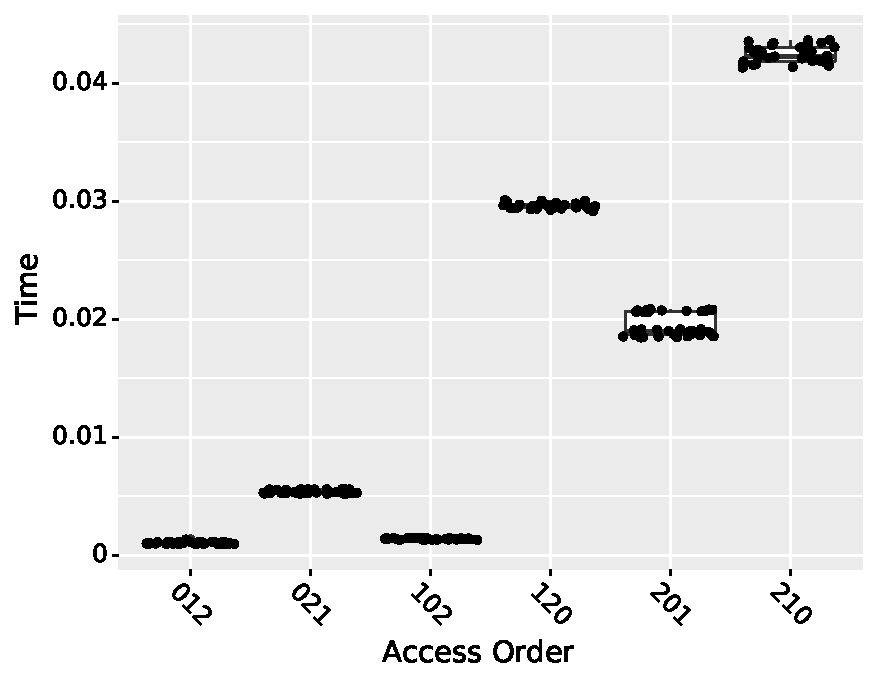
\includegraphics[width=\columnwidth]{benchmark1_boxplot.pdf}
	\caption{Execution times for 3-dimensional loop accessing 3-dimensional view, grouped by access order.}
	\label{AccessBenchmark1}
	\Description[Access Order Execution Times for Microbenchmark 1]{Fully described in the text.}
\end{figure}

\begin{figure}
	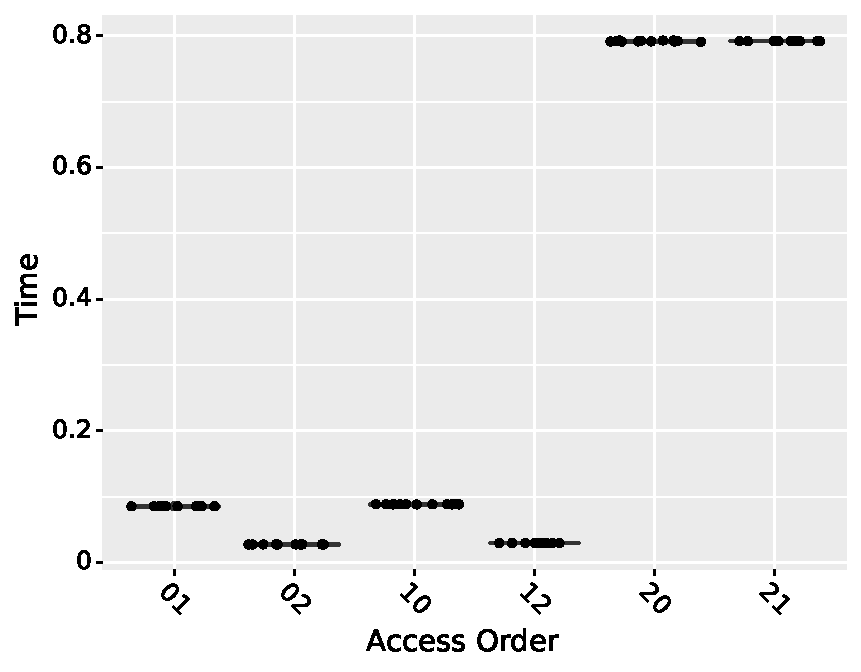
\includegraphics[width=\columnwidth]{benchmark2_boxplot.pdf}
	\caption{Execution times for 3-dimensional loop accessing 2-dimensional view, grouped by access order.}
	\label{AccessBenchmark2}
\end{figure}

\begin{figure}
	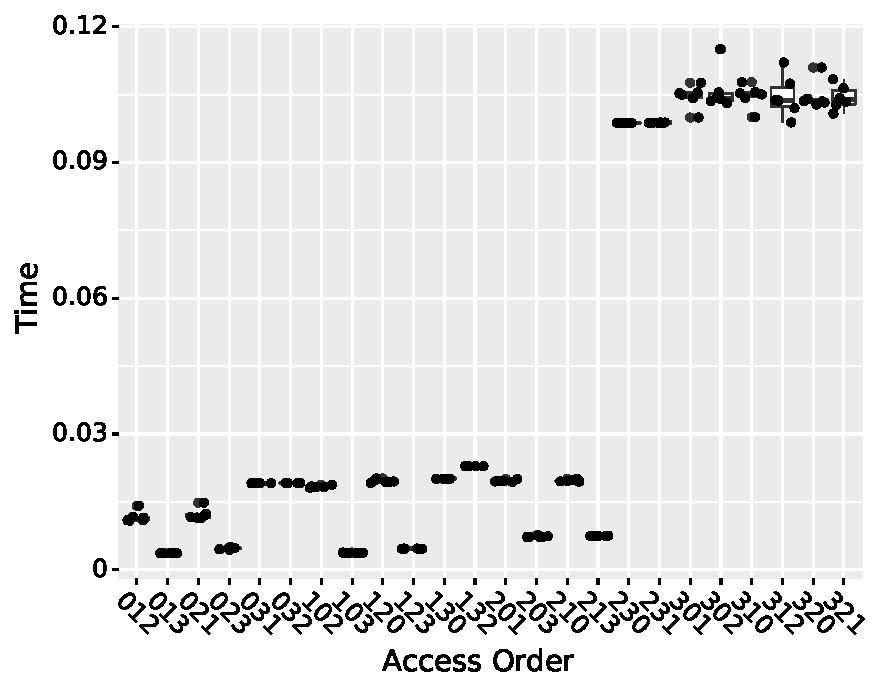
\includegraphics[width=\columnwidth]{benchmark3_boxplot.pdf}
	\caption{Execution times for 4-dimensional loop accessing 3-dimensional view, grouped by access order. \todo{Right now this isn't modulating argument order.}}
	\label{AccessBenchmark3}
\end{figure}

Figure~\ref{AccessBenchmark1} shows the execution times for the different access orders for microbenchmark 1.
Overall, the six possible access orders show good differentiation and clustering.
The access order $(2,0,1)$ does show two subclusters, but remain highly distinct from the other access order groupings. 
Additionally, access orders $(0,1,2)$ and $(1,0,2)$ show some overlap, likely because the bulk of the performance improvement comes from the innermost loop in a nest traversing the stride-one dimension of the data.

Figure~\ref{AccessBenchmark2} shows the execution times for the different access orders for microbenchmark 2. 
This microbenchmark also shows good cluster and differentiation.
Like microbenchmark 1, the access orders $(0,2)$ and $(1,2)$ have similar performance, likely for the same reason. 

Figure~\ref{AccessBenchmark3} shows the execution times for the different access orders for microbenchmark 3.
\todo{I need to finish reimplementing this one.}.
\begin{comment}


\todo{Brandon, I am not seeing these figures right now.  Have they not been included into the repository yet?}
Figure~\ref{accessBenchmark2} shows the execution times for the different access orders for microbenchmark 2. 
While the access orders for this microbenchmark are all highly clustered, they are less differentiated from one another. 
For example, we see that the orders $(0,2)$ and $(1,2)$ have similar performance, as do $(2,0)$ and $(2,1)$. 
The similarity in performance is again attributable to the influence of the position of the innermost loop iterator. 



Figure~\ref{accessBenchmark3} shows the execution times for the different access orders for microbenchmark 3. 
A similar pattern as the previous microbenchmarks emerges here: grouping based on the position of the innermost iterator. 

The major benefit of using access order as a performance metric is its reusability. 
Because it condenses the policy, the layout, and the arguments used in the access into a single metric, the same benchmarking results can be used to estimate the cost of all three accesses within a matrix multiplication. 
Similarly, the benchmarking results for access orders gathered for one computation can be reused when modeling another computation.

\end{comment}
\section{Evaluation}

\todo{Where we evaluated}

We evaluate our contribution on three codes: the polybench suite\nc, Kripke\nc, and miniWeather\nc.


\subsection{Evaluation Metrics}
When evaluating our systems, we consider a number of metrics. 
First,  we measure the source lines of code (SLOC) added, removed, and changed to implement layout changes by hand and using our \FormatDecisions interface.
Second, we measure the relative performance improvement between implementing layout changes by hand and using \FormatDecisions. 
This result shows the cost of modeling overhead.
Third, we measure the accuracy of our model on its own by determining the rank of its choices among all possible choices.
\todo{The explanation of the model accuracy measurement needs work.} 

\subsection{Case Study 1: Polybench}

Our first evaluation targeted select benchmarks from the polybench suite: 2mm, 3mm, gemver, and mvt.
For each benchmark, we implemented five variants.
\verb.RAJA_OpenMP. is the original RAJA implementation.
\verb.RAJALC. modifies \verb.RAJA_OpenMP. to use RAJALC kernel objects.
\verb.Hand_Layout., \verb.Format_Decision., and \verb.Model_Choice. all augment the \verb.RAJALC. variant to include format changes.
Table~\ref{VariantDescription} describes them in more detail.

\begin{table}
	\centering
	\begin{tabular}{ p{2.4cm} | p{1.1cm} | p{1.1cm} | p{1cm} | p{1cm}}
		Variant \linebreak Name & Kernel Objects & Layout Changes & Chosen \linebreak By & Written \linebreak Using \\
		\hline
		\verb.RAJA_OpenMP. & No & No & - & - \\
		\verb.RAJALC. & Yes & No & - & - \\
		\verb.Hand_Layout. & Yes & Yes & User & No API \\
		\verb.Format_Decision. & Yes & Yes & User & API \\
		\verb.Model_Choice. & Yes & Yes & Model & API
	\end{tabular}
	\caption{Polybench variant descriptions.}
	\label{VariantDescription}
\end{table}




\begin{table}
	\centering
	\begin{tabular}{c|c|c}
		Kernel & Variant & Layout Changes \\
		2MM & \verb.Hand_Layout. & Bview and Cview \\
		3MM & \verb.Hand_Layout. & Bview, Dview, Fview (2x) \\
		GEMVER & \verb.Hand_Layout. & None \\
		MVT & \verb.Hand_Layout. & None 
	\end{tabular}
\end{table}



\todo{This table is temporary.}
\begin{figure*}
\begin{tabular}{lll}
Benchmark   & Inclusion  & Implementation Status?\\
2mm         & Yes        &  \verb.RAJA_OpenMP., \verb.RAJALC., \verb.Hand_Layout.\\
3mm         & Yes        &  \verb.RAJA_OpenMP., \verb.RAJALC., \verb.Hand_Layout.\\
adi         & No, negative iterator increments       \\
atax        & No, accesses to A are in-order.          \\
bicg        & No, accesses to A are in-order.          \\
cholesky    & No, accesses to A are in-order.          \\
correlation & No, segs are in terms of other segs         \\
covariance  & No, segs are in terms of other segs          \\
deriche     & No, accesses to all multi-dimensional data are in-order.          \\
doitgen     & no, imperfect nesting        \\
durbin      & No, all 1D data.          \\
fdtd-2d     & No, accesses to all multi-dimensional data are in-order.           \\
floyd-warshall & No, accesses are in order \\
gemm        &  No, accesses are all in order         \\
gemver      & Yes        & \verb.RAJA_OpenMP. \verb.RAJALC. \verb.Hand_Layout. \\
gesummv     & No, accesses are all in order          \\
gramschmidt & No, imperfect nesting          \\
heat-3d     & No, accesses are all in order            \\
jacobi-1D   & No, accesses are all in order           \\
jacobi-2D   & No, accesses are all in order           \\
lu          & No, segs are in terms of other segs         \\
ludcmp      & No, segs are in terms of other segs \\
mvt         & Yes        & \verb.RAJA_OpenMP. \verb.RAJALC. \verb.Hand_Layout.\\
nussinov    & No, too much control flow and function calls          \\
seidel      & No, accesses are all in order           \\
symm        & No, imperfect nesting           \\
syr2k       & No, segs are in terms of other segs         \\
syrk        & No, segs are in terms of other segs        \\
trisolv     & No, accesses are all in order           \\
trmm        & No, segs are in terms of other segs         
\end{tabular}
\caption{Polybench benchmarks inclusion and implementation status.}
\end{figure*}




\subsection{Case Study 2: miniWeather}

\subsection{Case Study 3: Kripke}

\section{Related Work}

Wolf and Lam~\cite{wolf1991data} develop a schedule-based algorithm for improving data locality. 
Implemented in the SUIF compiler, they use a combination of interchange, skewing, reversal, and tiling to minimize the reuse distance of the computation's data. 
Their approach does not change the order of data in memory, just the schedule of the loops accessing that data.
McKinley, Carr, and Tseng~\cite{mckinley1996improving} offer a similar approach based on schedule transformations, incorporating loop fusion as well.

Kennedy and Kremer~\cite{kennedy1995automatic} developed an approach for automatically selecting data layouts for distributed arrays within High Performance Fortran (HPF). 
The high level optimization framework is similar to ours: breaking the program into segments, constructing a search space of layouts for each segment, estimating the cost of each layout choice, and selecting one candidate for each segment so that overall cost is minimized. 
Because they target distributed arrays, their approach considers the alignment of arrays with each other \todo{confirm this, i'm not 100\% sure}, while our approach considers the direct striding costs of each array separately. 
Furthermore, their cost estimation is performed statically~\cite{bixby1994automatic}, while ours incorporates the results of dynamic, system-specific microbenchmarking.


Chen, Ozturk, and Kandemir~\cite{Chen2004ilp} develop a model of locality using a 0-1 ILP formulation. 
Their decision variables indicate mappings between data elements and memory as well as scheduling choices surrounding when data elements are accessed. 
In their formulation, each data element is considered independently, meaning each array element has its own decision variable. 
Furthermore they assume complete flexibility of data ordering in memory, meaning there are no restrictions on array data being stored together.

Unat et. al.~\cite{unat2017trends} review trends in HPC related to data locality. They provide a variety of definitions which we utilize in our work. However, their definition of traversal order is not quite in line with RAJA's layout types, as layout changes affect the traversal order without changing the indices used. 
\section{Conclusion}


\bibliographystyle{abbrv}
\bibliography{DataRAJALC}
\end{document}
